% Portuguese-BR vertion
\documentclass{report}

\usepackage{ipprocess}
% Use longtable if you want big tables to split over multiple pages.
% \usepackage{longtable}
\usepackage[utf8]{inputenc} 
\usepackage[brazil]{babel} % Uncomment for portuguese

\sloppy

\graphicspath{{./pictures/}} % Pictures dir
\makeindex
\begin{document}

\DocumentTitle{Documento de Arquitetura}
\Project{*Nome do Projeto*}
\Organization{Universidade Estadual de Feira de Santana (UEFS)}
\Version{Build 1.4}

\capa
\newpage
\newpage

%%%%%%%%%%%%%%%%%%%%%%%%%%%%%%%%%%%%%%%%%%%%%%%%%%
%% Revision History
%%%%%%%%%%%%%%%%%%%%%%%%%%%%%%%%%%%%%%%%%%%%%%%%%%
\chapter*{Histórico de Revisões}
  \vspace*{1cm}
  \begin{table}[ht]
    \centering
    \begin{tabular}[pos]{|m{2cm} |m{2cm}| m{6cm} | m{3cm}|} 
      \hline
      \cellcolor[gray]{0.9}
      \textbf{Date} & \cellcolor[gray]{0.9} \textbf{Versão}  &\cellcolor[gray]{0.9}\textbf{Descrição} & \cellcolor[gray]{0.9}\textbf{Autor(s)}\\
      \hline
      22/03/2015 & 1.0 & Concepção e estruturação do Documento & Patrícia Gomes e Pedro Mota \\ \hline      
      26/03/2015 & 1.1 & \textit{Stakeholders} & Patrícia Gomes \\ \hline
      26/03/2015 & 1.2 & Adição do conjunto de componentes utilizados na concepção do jogo & Patrícia Gomes \\ \hline
	  28/03/2015 & 1.3 & Adição do datapath do gerador de números aleatórios & Kelvin Carmo \\ \hline      
      28/03/2015 & 1.4 & Descrição da Arquitetura & Alexandre Cavalcanti e Jhone Mendes \\ \hline
      29/03/2015 & 1.5 & Finalização dos tópicos e revisão & Alexandre Cavalcanti \\ \hline
    \end{tabular}
  \end{table}

% TOC instantiation
\tableofcontents

%%%%%%%%%%%%%%%%%%%%%%%%%%%%%%%%%%%%%%%%%%%%%%%%%%
%% Document main content
%%%%%%%%%%%%%%%%%%%%%%%%%%%%%%%%%%%%%%%%%%%%%%%%%%
\chapter{Introdução}
  
  \section{Propósito do Documento}
  Este documento descreve a arquitetura do projeto *Nome do Projeto*, "incluindo especificações dos circuitos internos, além da máquina de estados e o datapath do sistema. O documento apresenta também os módulos funcionais e como eles interagem entre si, assim como as definições de entrada e saída. O principal objetivo deste documento é definir as especificações do projeto e prover uma visão geral do mesmo."

  
  \section{Stakeholders}
    \FloatBarrier
    \begin{table}[H] 
      \begin{center}
        \begin{tabular}[pos]{|m{6cm} | m{8cm}|} 
          \hline 
          \cellcolor[gray]{0.9}\textbf{Nome} & \cellcolor[gray]{0.9}\textbf{Papel/Responsabilidades} \\ \hline
          Alexandre Cavalcanti, Fábio Barros, Jhone Mendes, Jussara Machado, Kelvin Carmo, Lucas Morais, Patricia Gomes, Pedro Mota & Desenvolvimento\\ \hline
          Jussara Machado, Fábio Barros, Kelvin Carmo & Implementação\\ \hline
          Lucas Morais, Pedro Mota & Testes\\ \hline
          Patrícia Gomes, Jhone Mendes, Alexandre Cavalcanti & Confecção da documentação\\ \hline
        \end{tabular}
      \end{center}
    \end{table} 

\section{Visão Geral do Documento}

O presente documento é apresentado como segue:
  
  \begin{itemize}
  \item \textbf{Sessão 2 -} Apresenta uma visão geral do sistema de acordo com seus requisitos.
  \item \textbf{Sessão 3 -} Descreve detalhadamente a arquitetura, explanando os módulos e componentes do projeto.
  \item \textbf{Sessão 4 -} Descreve o funcionamento básico do sistema de controle.
  \end{itemize}


  % inicio das definições do documento
  \section{Definições}
    \FloatBarrier
    \begin{table}[H]
      \begin{center}
        \begin{tabular}[pos]{|m{5cm} | m{9cm}|} 
          \hline
          \cellcolor[gray]{0.9}\textbf{Termo} & \cellcolor[gray]{0.9}\textbf{Descrição} \\ \hline
          Datapath & Caminho de dados percorrido para a execução de uma instrução. \\ \hline
          GNR & Módulo responsável por gerar números aleatórios. \\ \hline
        \end{tabular}
      \end{center}
    \end{table}  
  % fim

  % inicio da tabela de acronimos e abreviacoes do documento
  \section{Acrônimos e Abreviações}
    \FloatBarrier
    \begin{table}[H]
      \begin{center}
        \begin{tabular}[pos]{|m{2cm} | m{12cm}|} 
          \hline
          \cellcolor[gray]{0.9}\textbf{Sigla} & \cellcolor[gray]{0.9}\textbf{Descrição} \\ \hline
            GNR & Gerador de Número Randômico \\ \hline
        \end{tabular}
      \end{center}
    \end{table}  
  % fim

\chapter{Visão Geral}

    Simon Says é um jogo que consiste em desafiar o jogador a acertar uma determinada sequência de cores que tem seus elementos gerados aleatoriamente pelo próprio jogo. As cores, neste protótipo proposto neste documento, são representadas por quatro leds. É esperado que o jogador digite corretamente a sequência indicada dentro de 5 segundos pressionando botões correspondes às cores exibidas. O jogo apresenta dois modos e quatro níveis de dificuldade.
    No modo 1 o próprio sistema gera a sequência de cores, no modo 2 o jodador é o responsável por gerar essa sequência. Em cada nível aumenta a sequência de cores geradas. O jogador poderá ver ainda a última sequência gerada que ficará armazenada na memória enquanto o dispositivo estiver ligado.
\paragraph{}
    O sistema conta com uma interface de software que produz os comandos para o hardware de forma que seja possível que o mesmo apresente as cores nos LEDs e compare a cor do botão pressionado pelo jogador com a cor mostrada na sequência.
\paragraph{}
    A figura 2.1 apresenta o modelo de arquitetura do Warmup cujos elementos serão descritos na sessão seguinte:
\paragraph{}

%\begin{figure}[h] \centering \includegraphics[width=1.2\textwidth]{DataPath1.jpeg} \caption{Datapath do Sistema} \label{fig:mesh1} \end{figure}
  

% inicio das descrições de arquitetura para cada componente do sistema
\chapter{Descrição da Arquitetura}

  Abaixo os blocos apresentados na Figura 2.1 serão descritos:

    
  \section{Divisor de Frequência}
  Devido a necessidade de contar os segundos em algumas partes do sistema, fez-se necessário o uso de 16 flip-flops do tipo JK formando um contador dos pulsos de clock da FPGA, de 50MHz. Na contagem, o bit mais significativo pulsa a 1Hz sendo o suficiente para o sistema. A sua saída de 1Hz é usada na memória (além do original de 50MHz) para a função de repetir a última sequência, pois os leds não devem piscar rápidos demais como também em um contador (modulo Counter) que conta seus pulsos.
  
    
 
    \section{Gerador de Número Aleatório}
  Módulo responsável por gerar uma sequência aleatória de 2 bits. O sinal de entrada "next" serve para solicitar uma nova sequência. O "randomize" para receber um vetor de bits como semente, para começar a gerar os bits. Por último a "start-over", que dá origem a uma nova semente para gerar os bits.
  
    \subsection{Datapath Interno}
    \paragraph{}
    
%    \begin{figure}[H] \centering \includegraphics[width=0.9\textwidth]{datapath_gnr.jpeg}                \caption{Módulo Gerador Randômico} \label{fig:mesh1} 
%\end{figure}
    
   
  \section{Controle de Acesso à Memória}
  
  Este módulo é responsável pelo controle de uso dos dados contidos na memória (módulo memory). Ele libera o fluxo entre a memória e o gerador randômico (GNR) permitindo que o código de uma nova cor (color code) seja armazenado, controlando também quando todos os dados devem ser apagados (new game). Por meio deste também, é feita a operação de exibição da última sequência.
  
    \subsection{Definições de Entrada e Saída}
     \begin{table}[H]
       \centering
        \begin{tabular}[pos]{|m{2cm} |m{2cm}| m{3cm} | m{5cm}|} 
         \hline
          \cellcolor[gray]{0.9}
           \textbf{Nome} & \cellcolor[gray]{0.9} \textbf{Tamanho}  &\cellcolor[gray]{0.9}\textbf{Direção} & \cellcolor[gray]{0.9}\textbf{Descrição}\\ \hline
                Resposta & 1 Bit & Saída & Resposta da comparação entre valor na memória e valor de entrada dado pelo usuário\\ \hline
                Códigos* & 2 Bits & Entrada & Valores de mudança de estado do Controller no que diz respeito a memória. 
Onde: 00 = Comparar
01 = Nova cor
10 = Última sequência
11 = Limpar memória
  \\ \hline
                Códigos** & 2 Bits & Saída & Operações com a memória. 
Onde: 00 = Pegar o código (color code)
01 = Nova cor
10 = Última sequência
11 = Limpar memória
 \\ \hline
                Código de Cores & 2 Bits & Entrada & Referente a cor do botão pressionado. \\ \hline
        \end{tabular}
       \end{table}
    
    
  \section{Memória}
  
    Módulo responsável por armazenar as sequências de cores na memória. São utilizadas 64 posições de memória, sendo que são seis bits de endereço e cada posição guarda dois bits.
    \subsection{Definições de Entrada e Saída}
    
      \begin{table}[H]
       \centering
        \begin{tabular}[pos]{|m{2cm} |m{2cm}| m{6cm} | m{3cm}|} 
         \hline
          \cellcolor[gray]{0.9}
           \textbf{Nome} & \cellcolor[gray]{0.9} \textbf{Tamanho}  &\cellcolor[gray]{0.9}\textbf{Direção} & \cellcolor[gray]{0.9}\textbf{Descrição}\\ \hline
                read-address & 5 & Entada & Endereço usado na leitura\\ \hline
                write-address & 5 & Entrada & Endereço usada na escrita  \\ \hline
                write-data & 2 & Entrada & Dado a ser escrito \\ \hline
                read-data & 2 & Saída & Dado que sai da memória \\ \hline
                read-enable & -- & Entrada & Habilitador da leitura \\ \hline
                write-enable & -- & Entrada & Habilitador da escrita \\ \hline
                reset & -- & Entrada & Limpa a memória \\ \hline
        \end{tabular}
       \end{table}
    
    \subsection{Datapath}
    
    \begin{figure}[H] \centering 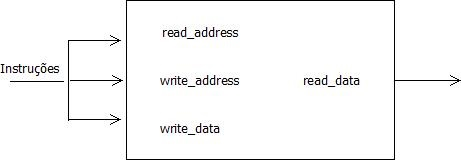
\includegraphics[width=0.9\textwidth]{memo.jpg} \caption{Datapath da memória} \label{fig:mesh1} \end{figure}
    
  \section{Contador}
  
  O contador é a unidade responsável por registrar o(s) intervalo(s) de tempo entre a(s) ação(ões) do jogador. Recebe o sinal de 1Hz do divisor de frequência afim de contar cinco segundos, que é o tempo que o jogador tem para apertar algum botão a partir do momento em que a sequência de comandos é gerada pelo GNR. No momento em que o um botão de cor é acionado o controller envia um sinal resetando o contador.
  
    \subsection{Definições de Entrada e Saída}
    
O contador possui duas entradas, sendo uma por onde chega o sinal proveniente do divisor de frequência e uma segunda entrada por onde o controller envia o sinal de reset, e possui uma saída enviando o sinal para o controller. A entrada e a saída são de 1bit.

   
  \section{Decodificador}
  
  O decodificador tem como função receber o dado referente a que cor deve "piscar" no jogo. Ele recebe uma(s) informação(ões) de dois bits da memória(que representa qual led deve "acender") e habilita o led correspondente.
  
    \subsection{Definições de Entrada e Saída}
    Possui uma entrada de dois bits(o valor binário vindo da memória) e quatro saídas de 1 bit.
    \paragraph{}
    
    
 \section{Controlador}
 O Controller é o módulo que representa o controlador, responsável por permitir a comunicação entre o \textit{software} e o \textit{hardware}. 
 As entradas do controlador são realizadas por quatro botões correspondentes às cores dos LEDs. Os botões podem ser pressionados tanto para reproduzir a sequência correta gerada pelo sistema, como para gerar a sequência no modo 2.
 \paragraph{}
   O modo e os níveis são escolhidos a partir de chaves de duas e quatro posições respectivamente e o botão \textit{Start} inicia o jogo. Além disso, existe também um botão responsável por apresentar a última sequência gerada.
 
    \subsection{Máquina de Estados}
    \begin{figure}[H] \centering 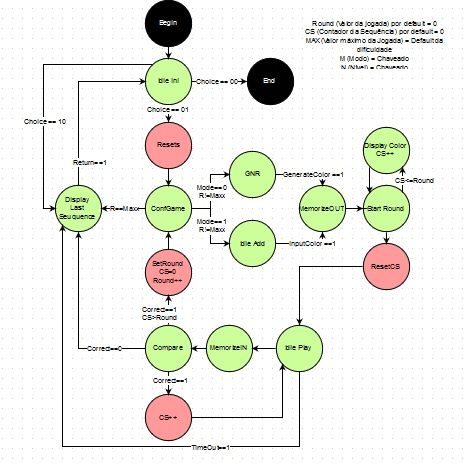
\includegraphics[width=0.9\textwidth]{Figura2.jpg}                \caption{Máquina de estados} \label{fig:mesh1} 
    \end{figure}
     
    
\chapter{Características}
    \section{Características Principais}
    A versão inicial do jogo possui as seguinte características:
     \begin{itemize}
        \item Mecanismo de controle modo de jogo e nível de dificuldade;
        \item Mecanismo de geração de sequência aleatória;
        \item Mecanismo de armazenamento da sequência gerada;
        \item Mecanismo de comparação da sequência gerada com a sequência armazenada;
        \item Comandos de controle formado a partir de um conjunto de operações.
      \end{itemize}
    
    \section{Comandos de Controle}
    O sistema de comandos para o jogo segue o padrão de codificação formado por dois bits como apresentado abaixo:
    \begin{table}[H]
       \centering
        \begin{tabular}[pos]{|m{2cm} |m{2cm}| m{6cm} | m{3cm}|} 
         \hline
          \cellcolor[gray]{0.9}
           \textbf{Código} & \cellcolor[gray]{0.9} \textbf{Descrição} \\ \hline
                00 & Compare \\ \hline
                01 & New Color \\ \hline
                10 & Last Sequence \\ \hline
                11 & Clean \\ \hline
                
        \end{tabular}
       \end{table}
       
    \section{Comandos de Resposta}
    O sistema de controle processa e transmite sinais de respostas que indicam as cores, apresentadas em forma de luz de LED.
    \begin{table}[H]
       \centering
        \begin{tabular}[pos]{|m{2cm} |m{2cm}| m{6cm} | m{3cm}|} 
         \hline
          \cellcolor[gray]{0.9}
           \textbf{Código} & \cellcolor[gray]{0.9} \textbf{Descrição} \\ \hline
                00 & LED vermelho \\ \hline
                01 & LED verde \\ \hline
                10 & LED amarelo \\ \hline
                11 & LED azul \\ \hline
                
        \end{tabular}
       \end{table}
    



% Optional bibliography section
% To use bibliograpy, first provide the ipprocess.bib file on the root folder.
% \bibliographystyle{ieeetr}
% \bibliography{ipprocess}

\end{document}
